\documentclass{jarticle}

\usepackage{graphicx}
\usepackage{url}
\usepackage{listings,jlisting}
\usepackage{ascmac}
\usepackage{amsmath,amssymb}

%ここからソースコードの表示に関する設定
\lstset{
  basicstyle={\ttfamily},
  identifierstyle={\small},
  commentstyle={\smallitshape},
  keywordstyle={\small\bfseries},
  ndkeywordstyle={\small},
  stringstyle={\small\ttfamily},
  frame={tb},
  breaklines=true,
  columns=[l]{fullflexible},
  numbers=left,
  xrightmargin=0zw,
  xleftmargin=3zw,
  numberstyle={\scriptsize},
  stepnumber=1,
  numbersep=1zw,
  lineskip=-0.5ex
}
%ここまでソースコードの表示に関する設定

\title{知能プログラミング演習II 課題2}
\author{グループ07\\
  29114007 池口 弘尚\\
%  {\small (グループレポートの場合は、グループ名および全員の学生番号と氏名が必要)}
}
\date{2019年10月7日}

\begin{document}
\maketitle

\paragraph{提出物} rep2
\paragraph{グループ} グループ07
\paragraph{メンバー}
\begin{tabular}{|c|c|c|}
  \hline
  学生番号&氏名&貢献度比率\\
  \hline\hline
  29114007&池口弘尚&0\\
  \hline
  29114031&大原拓人&0\\
  \hline
  29114048&北原太一&0\\
  \hline
  29114086&飛世裕貴&0\\
  \hline
  29114095&野竹浩二朗&0\\
\end{tabular}

\section{課題の説明}
\begin{description}
\item[課題2-1] MatchingクラスまたはUnifyクラスを用い,パターンで検索可能な簡単なデータベースを作成せよ.
\item[課題2-2] 自分たちの興味ある分野の知識についてデータセットを作り,上記2-1で実装したデータベースに登録せよ.また,検索実行例を示せ.どのような方法でデータセットを登録しても構わない.
\item[課題2-3] 上記システムのGUIを作成せよ.
\end{description}


\section{課題2-1}
\begin{screen}
  MatchingクラスまたはUnifyクラスを用い,パターンで検索可能な簡単なデータベースを作成せよ.
\end{screen}

DataBase,Data,SentenceAnalysisに関しては、私が担当した。

\subsection{手法}
配列から全探索すると、要素が増えれば増えるほど探索に時間がかかることが想定されたので、DataBaseを作りある程度候補を絞ってから探索するという手法を使用した。

\subsection{実装}
まず、新たに追加したクラスは以下の
\begin{itemize}
\item DataBaseクラス: 読み込んだ文字列をDataクラスとして保持しておくためのクラス。文字列の具体化されている部分から候補を絞る機能も持つ。
\item Dataクラス: 最初の名詞が同じものの文字列を保存しておくためのクラス。
\item SentenceAnalysisクラス: 文字列を最初の名詞と動詞周辺とそれ以外に分けるためのクラス。
\item Unifierクラス: 具体化されていない文字列を使用して探索を行うクラス。
\end{itemize}

SentenceAnalysisクラスにおける文字列を三分割するためのメソッドAnalysisは以下のように実装した。

\begin{lstlisting}[caption=SentenceAnalysisのAnalysis,label=src:Analysis]
static String[] Analysis(String sentence) throws NoSuchElementException {
	String[] elements = new String[3];
	StringTokenizer tokenizer = new StringTokenizer(sentence);
	elements[0] = tokenizer.nextToken();
	elements[1] = tokenizer.nextToken();
	elements[2] = "";
	while (true) {
		String t = tokenizer.nextToken();
        //前置詞が含まれていた場合はそれ以前を動詞部分に結合
		if (PrepositionCheck(t)) {
			if (elements[2] == "")
				elements[1] += " " + t;
			elements[2] += t;
			elements[1] += " " + elements[2];
			elements[2] = "";
		} else {
			elements[2] += t;
			if (tokenizer.hasMoreTokens())
				elements[2] += " ";
			else
				break;
		}
	}
	return elements;
}
\end{lstlisting}


Dataクラスは同じ名詞のデータを格納する機能を持っている。データの操作に関するinsert,remove,searchは以下のように実装した。
\begin{lstlisting}[caption=Dataのデータ操作関連のメソッド,label=src:DataControl]
//メンバ変数として持つ名詞部分とそれ以降
String name;
Map<Integer, List<String>> records;

//コンストラクタで名詞を設定
public Data(String name) {
	this.name = name;
	records = new HashMap<>();
}

//要素を追加
public void insert(int key, String value) {
	if (records.containsKey(key)) {
		records.get(key).add(value);
	} else {
		List<String> list = new ArrayList<>();
		list.add(value);
		records.put(key, list);
	}
}

//要素を削除
public boolean remove(int key, String value) {
	boolean result = false;
	List<String> list = records.get(key);
	if (list != null) {
		result = list.remove(value);
        //空になったらマップを削除
		if (list.isEmpty())
			records.remove(key);
	}
	return result;
}

//動詞付近で検索
public boolean Search(Collection<Integer> collection) {
	for (Integer integer : collection) {
		if (records.containsKey(integer))
			return true;
	}
	return false;
}

//後部で検索
public boolean Search(String value) {
	for (List<String> list : records.values()) {
		for (String s : list) {
			if (s==value)
				return true;
		}
	}
	return false;
}
\end{lstlisting}

上記のDataクラスを利用して、データを格納するクラスDataBaseクラスを実装してある。
DataBaseは常に自身のインスタンスを保持する。それを以下のように実装した。
\begin{lstlisting}[caption=DataBaseのインスタンス保持,label=src:DataBaseInstance]
public class DataBase {
	private static DataBase instance = new DataBase();
	Map<String, Data> datas;
	Map<String,Integer> keyMap;
	static int id = 0;

	//常に同じインスタンスを返す
	static DataBase getDataBase() {
		return instance;
	}
    ...
}
\end{lstlisting}

また、DataBaseのデータの操作に関するinsert,remove,searchは以下のように実装した。
\begin{lstlisting}[caption=DataBaseのデータ操作,label=src:DataBase]
//文の追加
boolean insert(String sentence) {
	String[] values = null;
    //具体化されていないものは読み込まない
	if(sentence.contains("?"))
		return false;
	try {
		values = SentenceAnalysis.Analysis(sentence);
	} catch (Exception e) {
		return false;
	}
	int key = -1;
	if (!keyMap.containsKey(values[1])) {
		keyMap.put(values[1],id++);
		key = keyMap.size() - 1;
	} else
		key = keyMap.get(values[1]);
	if (datas.containsKey(values[0])) {
		datas.get(values[0]).insert(key, values[2]);
	} else {
		Data data = new Data(values[0]);
		data.insert(key, values[2]);
		datas.put(values[0], data);
	}
	return true;
}

//文の削除
boolean remove(String sentence) {
	String[] values = null;
	try {
		values = SentenceAnalysis.Analysis(sentence);
	} catch (Exception e) {
		return false;
	}

	int key = keyMap.get(values[1]);
	if (key != -1) {
		Data data = datas.get(values[0]);
		if (data.remove(key, values[2])) {
			if (data.records.isEmpty())
				datas.remove(values[0]);
			return true;
		}
	}
	return false;
}

//名詞部分で候補を絞る
DataBase searchByName(String name) {
	DataBase dataBase = new DataBase();
    //データのインスタンスは作成しない
	Data d = datas.get(name);
	if (d == null)
		return null;
	Set<Integer> keyset =d.records.keySet();
	for (String s : keyMap.keySet()) {
		if(keyset.contains(keyMap.get(s)))
			dataBase.keyMap.put(s, keyMap.get(s));
	}
	dataBase.datas.put(name, d);
	return dataBase;
}

//文で検索
DataBase Search(String sentence) {
	DataBase dataBase = this;
	String[] values = null;
	try {
		values = SentenceAnalysis.Analysis(sentence);
	} catch (Exception e) {
		return null;
	}
    //具体化されている部分から候補を絞る
	if (!isVar(values[0]))
		dataBase = dataBase.searchByName(values[0]);
	if (!isContainVar(values[1]))
		dataBase = dataBase.searchByVarb(values[1]);
	if (!isContainVar(values[2]))
		dataBase = dataBase.searchByValue(values[2]);
	return dataBase;
}
\end{lstlisting}

これら以外に関してはグループレポートを参照。

\subsection{実行例}
追加したデータ

Hanako is a girl

Jiro loves Hanako


検索した文字列

?x is a girl;?z loves ?x

\{?x=Hanako, ?z=Jiro\}


削除した文字列

Jiro loves Hanako

検索した文字列

?x is a girl;?z loves ?x

検索失敗
\subsection{考察}
データベースに関しては、全体として1つしか実体を持たないため、疑似シングルトンパターンを使用した。
これは、候補を絞るときにDataBaseそのものを返した方が都合が良いためそのような実装となった。
DataBaseの特徴としては、文を三分割して保存するということもそうだが、最も気を付けて作った部分は検索するときにDataのインスタンスに手を加えないことによって、Dataを新しく作らなくても絞った後のDataBaseを形成することができるという点である。
DataBaseのインスタンスを作成したとしても、Dataを使いまわしていればメモリの消費を抑えることができる。

絞り込むプロセスとしては、三分割した中で具体化されている部分のみを使用して絞り込んでいる。
しかし、実際にはこのプロセスで文全体を一度見回しているため、この段階で具体化もしておいた方がより効率よく探索できると考えられる。

また、最後の部分での絞り込みにおいては、Dataの中身を変えることができないため、十分に絞ることができなかった。
これはSearchがDataBase型で返しているために実装ができなくなってしまうが、List<String>で返すことによって解決できる可能性がある。



\section{課題2-2}
\begin{screen}
  自分たちの興味ある分野の知識についてデータセットを作り,上記2-1で実装したデータベースに登録せよ.また,検索実行例を示せ.どのような方法でデータセットを登録しても構わない.
\end{screen}

担当していないためグループレポートを参照。


\section{課題2-3}
\begin{screen}
  上記システムのGUIを作成せよ
\end{screen}

発展問題に関しては、私が担当した。

\subsection{手法}
swingのカードレイアウトを使用して、それぞれの機能をパネル分けし、大きなパネルで扱うことができるように実装した。

\subsection{実装}
まず、新たに追加したクラスは以下の
\begin{itemize}
\item FrameBaseクラス: JFrameを継承。コンストラクタのみ実装しており、JFrameの各種設定が1行でできるようにしてある。rep1と同じ。
\item MakeGUIFrameクラス: GUIの型を作成するためのクラス。
\item AddPanel,SearchPanel,RemovePanelクラス: JPanelを継承。各種パネルを描画するためのメソッドが実装されている。
\item TextLogクラス: JScrollPaneを継承。ビューポートにJTextAreaを持ち、ログを表示するためのクラス。
\item TxtFilterクラス: FileFilterを継承。JFileChooserのフィルタ。
\end{itemize}

MakeGUIFrameにおけるカードレイアウトは以下のように実装した。


\begin{lstlisting}[caption=GUI作成,label=src:MakeGUIFrame]
public static void MakeMatchingGUI() {
	FrameBase frame = new FrameBase("test", 1000, 500);
	JPanel cardPanel;
	CardLayout layout;
	/* カード1 */
	AddPanel card1 = new AddPanel();

	/* カード2 */
	SearchPanel card2 = new SearchPanel();

	/* カード3 */
	RemovePanel card3 = new RemovePanel();

	//cardPanelにカードレイアウトをセット
	cardPanel = new JPanel();
	layout = new CardLayout();
	cardPanel.setLayout(layout);

	cardPanel.add(card1, "Add");
	cardPanel.add(card2, "Search");
	cardPanel.add(card3, "Remove");

	ActionListener listener = new ActionListener() {

		@Override
		public void actionPerformed(ActionEvent e){
			String cmd = e.getActionCommand();

			switch (cmd) {
			case "Add":
			case "Search":
			case "Remove":
            	//ページの切り替え
				layout.show(cardPanel, cmd);
				break;
			case "Save":
				Save(frame);
				break;
			case "Exit":
				System.exit(0);
				break;
			default:
				System.out.println("ボタンの割り当てが存在しない");
				break;
			}
		}
	};
    ...
}
\end{lstlisting}

カードパネルに乗せるパネルであるAddPanel,SearchPanel,RemovePanelの基本的な構造は同じで、ボタンをクリックしたときに、テキストボックスに入れられた文字を読み取って処理するだけなので説明は省く。
ただ、AddPanelにはファイルを参照して読み込む機能が以下のように実装されている。
\begin{lstlisting}[caption=ファイルの参照,label=src:FileChooser]
//参照ボタンのActionListener
ActionListener listener2 = new ActionListener() {

	@Override
	public void actionPerformed(ActionEvent e) {
    	//カレントディレクトリのパスを得る
		String path = System.getProperty("user.dir");
		JFileChooser filechooser = new JFileChooser(path);
        //フィルタを追加
		filechooser.setFileFilter(new TxtFilter());
		int selected = filechooser.showOpenDialog(p2);
		if (selected == JFileChooser.APPROVE_OPTION) {
			File file = filechooser.getSelectedFile();
			adress.setText(file.getAbsolutePath());
		}
	}
};
\end{lstlisting}

また、それぞれのパネルでのログを表示するためにTextLogを以下のように実装した。
\begin{lstlisting}[caption=TextLog,label=src:TextLog]
class TextLog extends JScrollPane {
	JTextArea area;
	JViewport viewport;

	public TextLog(int rows, int columns) {
		super();
		area = new JTextArea(rows, columns);
		EtchedBorder border = new EtchedBorder(EtchedBorder.RAISED);
		area.setEditable(false);
		area.setBorder(border);
		setViewportView(area);
		viewport = getViewport();
	}

	//ログを1行分書き込む
	public void addLog(String txt) {
		area.append(txt + "\n");
	}
}
\end{lstlisting}



\subsection{実行例}
実行すると次のようなGUIが表示される。


\begin{figure}[!hbt]
  \centering
  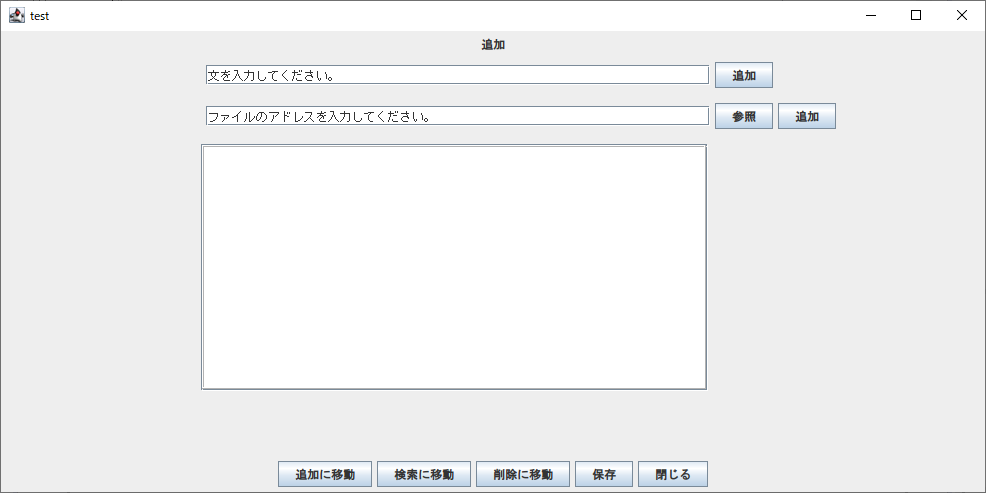
\includegraphics[bb=0 0 986 493,width=1.2\linewidth]{pic1.png}
  \caption{追加のGUIパネル}
  \label{fig:pic1}
\end{figure}

上のテキストボックスを利用すれば、1文ずつデータベースに追加することができる。下の参照をクリックすると次のように表示される。

\begin{figure}[!hbt]
  \centering
  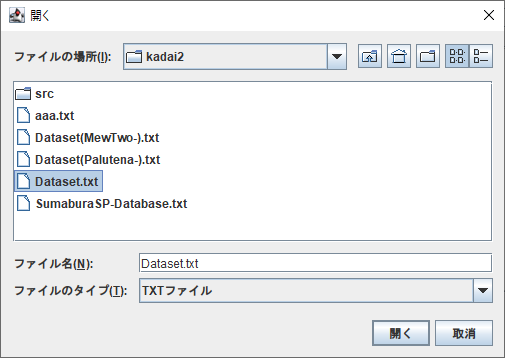
\includegraphics[bb=0 0 505 358,width=1\linewidth]{pic2.png}
  \caption{読み込むファイルを参照}
  \label{fig:pic2}
\end{figure}

これでデータセットの.txtを開くと自動的にpathが入力され、追加を押せばデータセットを読み取ってくれる。

検索パネルでは、検索する文を;で区切って入力することによって複数の文を検索することができる。

\begin{figure}[!hbt]
  \centering
  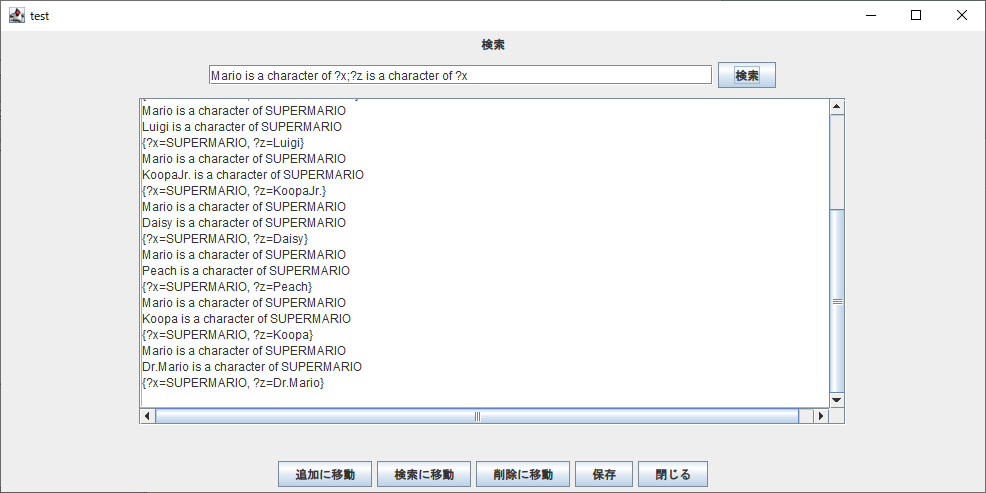
\includegraphics[bb=0 0 986 493,width=1.2\linewidth]{pic4.png}
  \caption{検索のGUIパネル}
  \label{fig:pic4}
\end{figure}

削除パネルでは入力した文をデータベースから取り除くことができる。また、検索時のように具体化されていない値を用いることによって一括で削除することもできる。

\begin{figure}[!hbt]
  \centering
  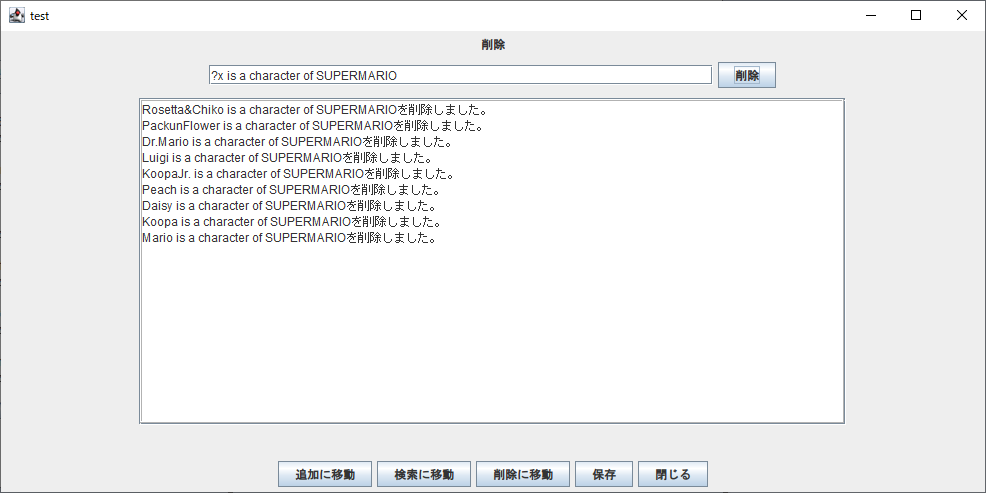
\includegraphics[bb=0 0 986 493,width=1.2\linewidth]{pic5.png}
  \caption{削除のGUIパネル}
  \label{fig:pic5}
\end{figure}

また、保存ボタンを押すと現在のデータベースを.txtで保存することができる。
\begin{figure}[!hbt]
  \centering
  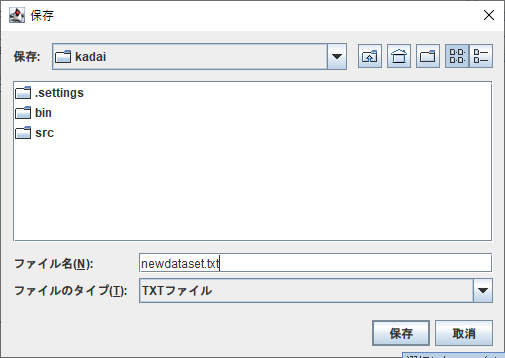
\includegraphics[bb=0 0 505 358,width=1\linewidth]{pic7.png}
  \caption{保存}
  \label{fig:pic7}
\end{figure}

\subsection{考察}
前回に引き続き、swingでGUIを作成した。

今回のプログラムの実装では、前回のものよりも出来ることの選択肢が増えているため、操作をGUI化することによって大きな恩恵を受けることができるように思われる。
コマンドで実行することを考えるとかなり操作が複雑化しそうなところを上手く簡単化できたと思う。
それぞれの操作をパネルで分けることによって、操作の切り替えが分かりやすくなるようにしている。
ただ、コマンドではエンターを押すだけで操作を進めることができたが、GUIではそれを行うことができない。

\section{感想}
GUIを作成するのは2度目のため、実装にそれほど時間はかからなかった。
そのため、発展ではない課題にも取り組んだが、勝手に進めていってしまったため、他のメンバーがするべき作業を取ってしまったように思う。
また、データベースクラスの仕様をしっかり決めずに実装に取り組んでしまったため、チームメイトがそれを利用したプログラムを書くのが遅くなってしまった。
そのため、わかる範囲でメソッドの仕様の共有をする必要があると思った。


% 参考文献
\begin{thebibliography}{99}
\bibitem{swing} Swingを使ってみよう - Java GUIプログラミング
\url{https://www.javadrive.jp/tutorial/} (2019年10月21日アクセス).


\end{thebibliography}

\end{document}